\section{Discussion} \label{sec:discussion}

%%%%%%%%%%%%%%%%%%%%%%%%%%%%%%%%%%%%%%%%%%%%%%%%%%%%%%%%%%%%%%%%%%%%%%%%%%%%%%%%
\subsection{Degenerate cases}

\begin{figure} %[!ht]
    \centering
    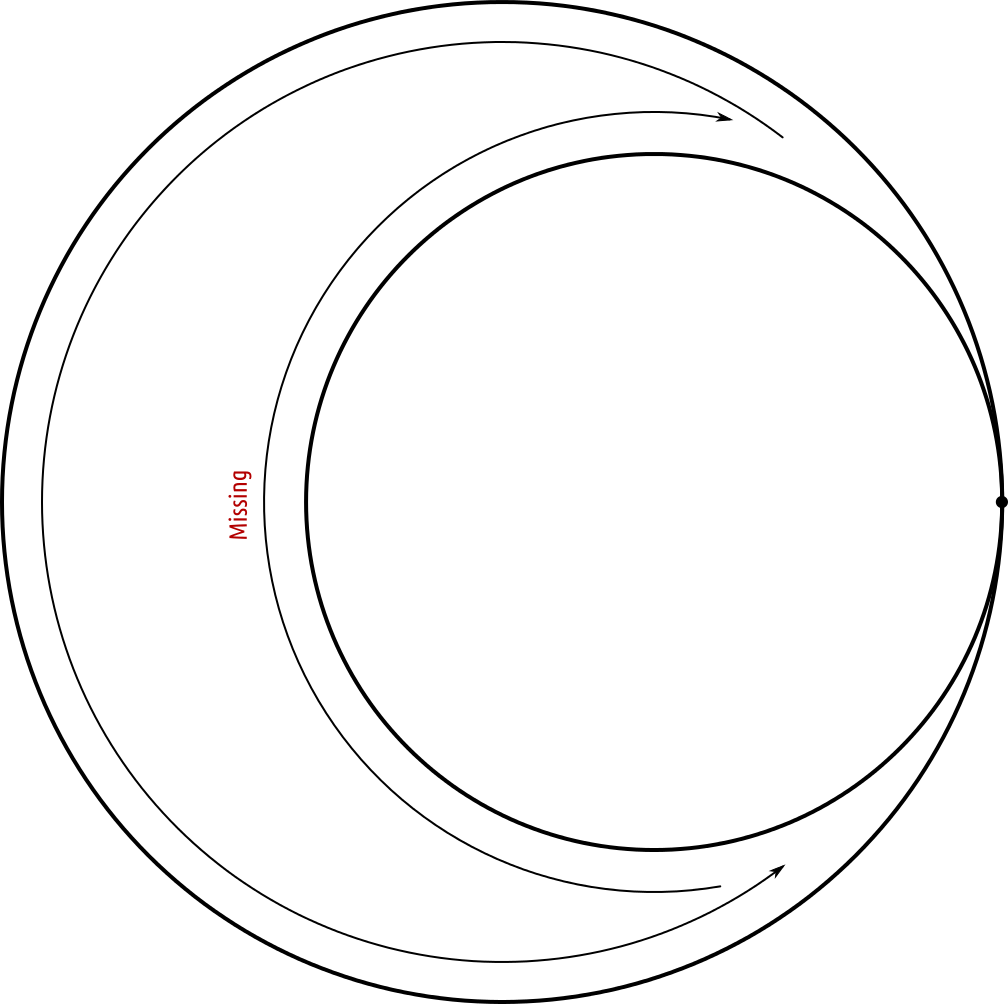
\includegraphics[width=.5\textwidth]{figures/disc_specialCase1.png}
    \caption{xxx}
    \label{fig:disc_specialCase1}
\end{figure}


%%%%%%%%%%%%%%%%%%%%%%%%%%%%%%%%%%%%%%%%%%%%%%%%%%%%%%%%%%%%%%%%%%%%%%%%%%%%%%%%
\subsection{Future work}


%%%%%%%%%%%%%%%%%%%%%%%%%%%%%%%%%%%%%%%%
\subsubsection{Beyond straight lines and circles}

Do we need them? aren't circle and line sufficient for geometric abstraction?

%%%%%%%%%%%%%%%%%%%%%%%%%%%%%%%%%%%%%%%%
\subsubsection{Dynamic subdivision}
%% 1) moving curves: Find ``some conditions'' where as long as they are satisfied, the subdivision maintains the same graph structure, hence the same subdivision.
%% These conditions must be fast to compute (intersection processes is too slow)
%% Could these conditions provide measures for updating the geometry of the subdivision (i.e. attriubutes of nodes and edges).
%% recompute the subdivision
%% 2) adding/removing curves


%%%%%%%%%%%%%%%%%%%%%%%%%%%%%%%%%%%%%%%%
\subsubsection{Face merging, a case of constructive geometry}
